%%%%%%%%%%%%%%%%%%%%%%%%%%%%%%%%%%%%%%%%%%%%%%%%%%%%%%%%%%%%%%%%%%%%%%%%%%%%%%%%%%%%%%%%%%%%%
%%									   Chapitre 2	    								 %%
%%%%%%%%%%%%%%%%%%%%%%%%%%%%%%%%%%%%%%%%%%%%%%%%%%%%%%%%%%%%%%%%%%%%%%%%%%%%%%%%%%%%%%%%%%%%%
\chapter{Modélisation  du système}
\minitoc
\newpage
%%%%%%%%%%%%%%%%%%%%%%%%%%%%%%%%%%%%%
\section{Introduction}
Tous les programmes informatiques n’ont pas été construits à l’aveuglette par les
programmeurs, même les plus petits ont fait l’objet de quelques réflexions. Pour notre cas,
quelques réflexions ne suffisent pas, il en faut beaucoup. Mais on peut facilement se perdre
dans ces réflexions si on n’a pas de méthodes et un langage de modélisation bien adaptée. Nous construisons des modèles de systèmes complexes parce nous sommes incapables d'appréhender ces systèmes dans leur entièreté.
 Mais c'est quoi vraiment  un modèle?
\medskip
	  Un modèle est une simplification de
	  la réalité. la modélisation permet alors de maitriser
	  la complexité du système étudié,
	  car chaque modèle donne accès à
	  une représentation abstraite de
	  différents aspects du système.
	modéliser un système   consiste à créer une représentation schématique simplifié d'un problème. Le but est de:
	\begin{itemize}
\item Nous aider à visualiser le système tel qu'il est ou tel qu'il devrait être.
\item Spécifier la structure et le comportement d'un système
\item Avoir un "patron" pour guider la construction du système.
\item Documenter les décisions qui ont été prises
	\end{itemize}
	

	
	% %eventuellement uml definition les diagrame  presentation merise pour la base de donne uml pour la modeleisation
	
	
	
	
	
	
	
	
	
	
	
	
	
	
	
	
	
	
	
	
	
	
	
	
	\section{Quelque notion sur la modélisation UML}
	
	\newpage
	\section{Spécification de besoin}
	Pour se lancer dans la modélisation, on a besoin des information concernant cette établissement sanitaire pour comprendre le mécanisme qui y se trouve.
	De façon générale, le fonctionnement de l'hôpital repose sur l'ordonnancement des
	branches ci dessous.
	
	\subsection{Besoin de l'accueil }
	Un nouvel arrivant dans le centre hospitalier doit impérativement se présenter à l'accueil.
	De là, le responsable a besoin d'enregistrer les renseignements de base du nouveau malade, à
	savoir :
	La date d'entrée, le nom Prénom, le sexe, l'age, l'adresse, le téléphone, le médecin traitant, la famille ou personne externe,  la profession et l'unité d'admission.
	 Sur l'unité d'admission, ceci est à propos du département dans lequel le patient va être orienté
	Il est à noter que les renseignements sus enregistrés, feront l'objet d'une fiche qui
	sera remplie au fur et à mesure du traitement du patient concerné, une fois admis
	dans l'unité d'admission
	
	\medskip
	
	Quand un malade doit être hospitalisé, c'est également à l'accueil que cet évènement
	doit être pris en compte. En effet, le responsable enregistre :
	
	Le numéro du patient (entre autre, son dossier médical), la chambre le lit et la catégorie de la chambre
	
	\medskip
	Comme le rôle de l'accueil se repose surtout sur l'enregistrement du mouvement de la	population hospitalière, à la sortie d'un patient, un personnel de l'accueil enregistre la	sortie, avec les attributs suivants :
	le numéro de patient	le nom et prénom, l'état de sortie (mort, guérison, amélioration, statu-quo), la décision de sortie (de l'hôpital ou volontaire)




\subsection{ départements d'admission}

A La polyclinique Universitaire NEXT, on retrouve les départements suivants :

la maternité, chirurgie,bloc, opératoire,        néphrologie,  pédiatrie, gynécologie, mise en observation.

Une fois que le patient est orienté vers son unité d'admission, la département  a besoin de modifier la  fiche médical du malade, en
rapport avec son suivi médical.


\subsection{L'administration}

Toutes les prestations effectuées par le patient sont notées et enregistrées par un
responsable de administration.L'administration a besoin d'enregistrer toutes les prestations.


\subsection{La caisse}
La caisse est chargée du service facturation. Quand un patient va passer au paiement, il se
présente à la caisse. Le caissier consulte les prestations saisies par l'administration.
Son rôle vise également à l'évaluation et l'exploitation d'un certain nombre d'informations
et de statistiques, liées à la comptabilité des prestations.

\subsection{La direction}
La direction a dans ses attributs, la gestion des utilisateurs, la diffusion
d'informations/messages au personnel.

\subsection{La médecine}

La section médecine est dédiée aux médecins, plutôt dans le sens de prescription. Quand un
patient se présente alors au cabinet, le médecin lui prescrit une ordonnance









	\newpage
	
	
	
	
	
	
	
	
	
	
	
	\section{Diagrame de cas d'utilisation}
	
	\subsection{Diagramme de cas d'utilisation générale du systéme}
	\begin{figure}[h]
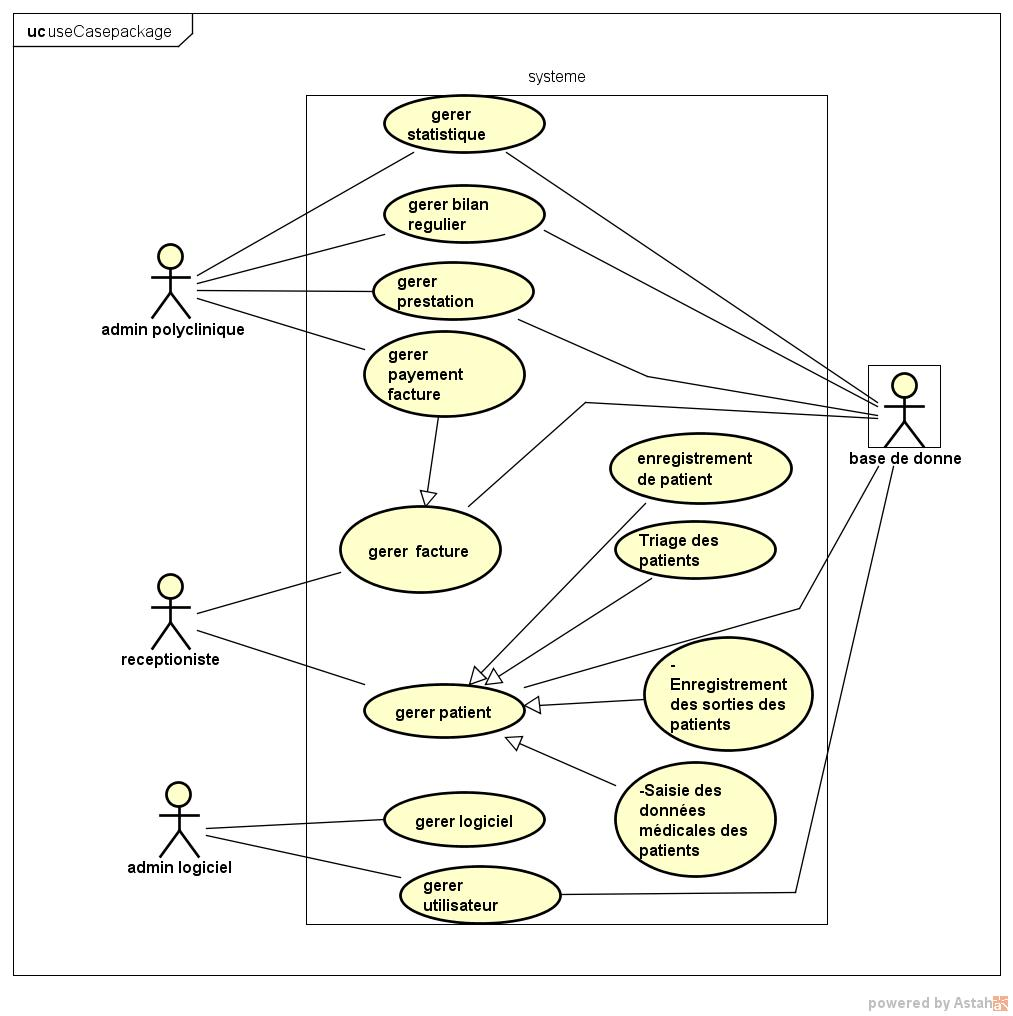
\includegraphics[scale=0.5]{Chapitre2/images/mainUseCaseDiagramme.jpg}
\caption{Diagramme de cas d'utilisation générale du systéme}
	\end{figure}
	
\newpage

	\subsection{Diagramme de cas d'utilisation réceptionniste }
	  
	  \begin{figure}[h]
	  \centering
	   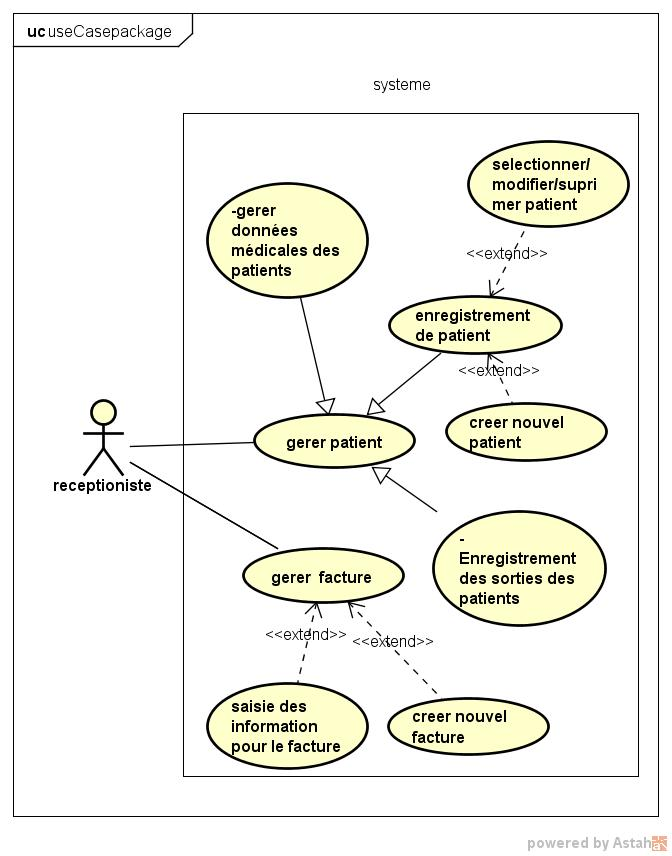
\includegraphics[scale=0.5]{Chapitre2/images/ucdreceptioniste}
	    \caption{Diagramme de cas d'utilisation réceptionniste}
	  \end{figure}
	 
\newpage

	\subsection{Diagramme de cas d'utilisation administrateur polyclinique }
	  
	  \begin{figure}[h]
	  \centering
	  
	   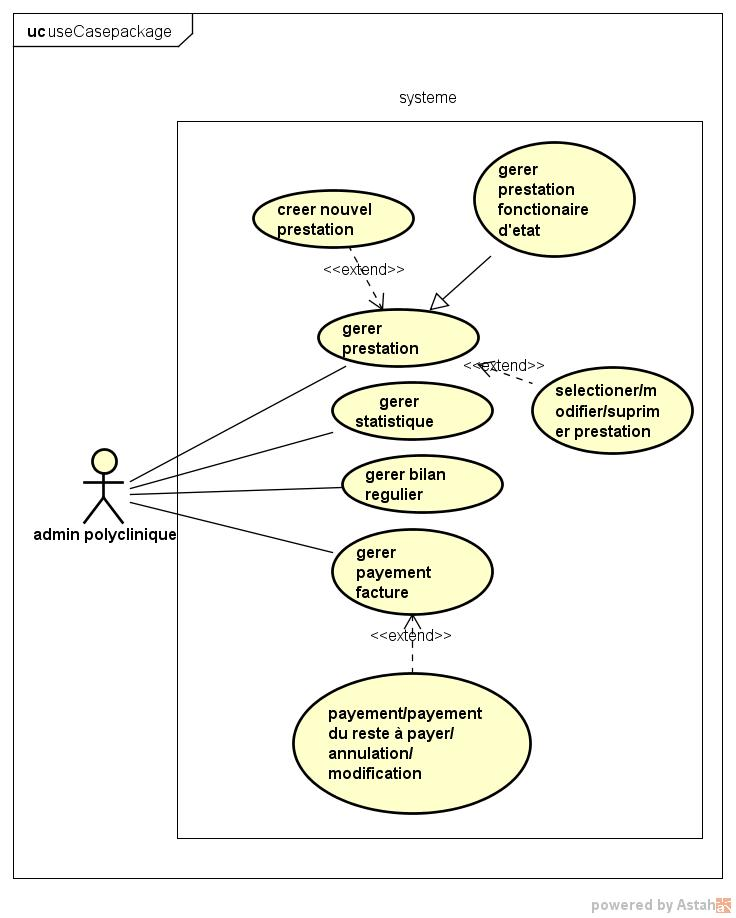
\includegraphics[scale=0.5]{Chapitre2/images/ucdadminPolyclinique.jpg}
	    \caption{Diagramme de cas d'utilisation administrateur polyclinique }
	  \end{figure}
	 
\newpage

	\subsection{Diagramme de cas d'utilisation admin logiciel}
	  
	  \begin{figure}[h]
	  \centering
	   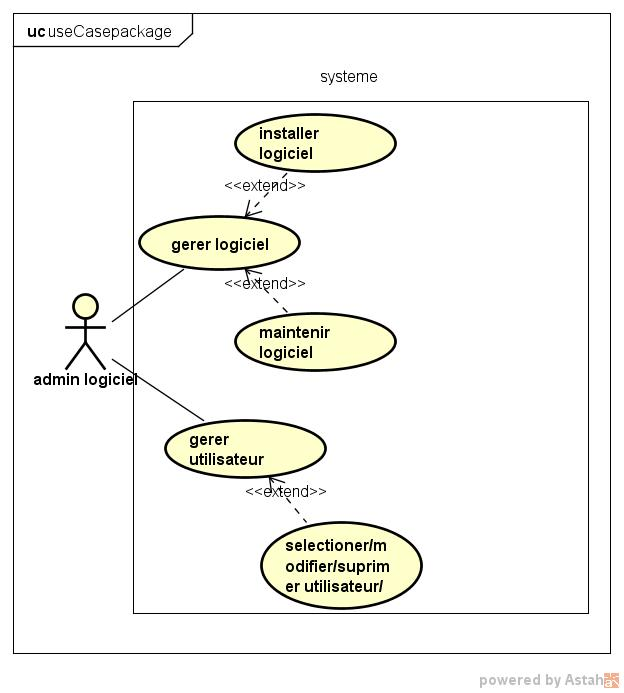
\includegraphics[scale=0.6]{Chapitre2/images/ucdadminlogiciel}
	    \caption{Diagramme de cas d'utilisation administrateur logiciel}
	  \end{figure}
	 
	  \newpage
	  
	  \section{diagramme de séquence}
	  
	   \subsection{Diagramme de séquence authentification}
	  	  \begin{figure}[h]
	  	  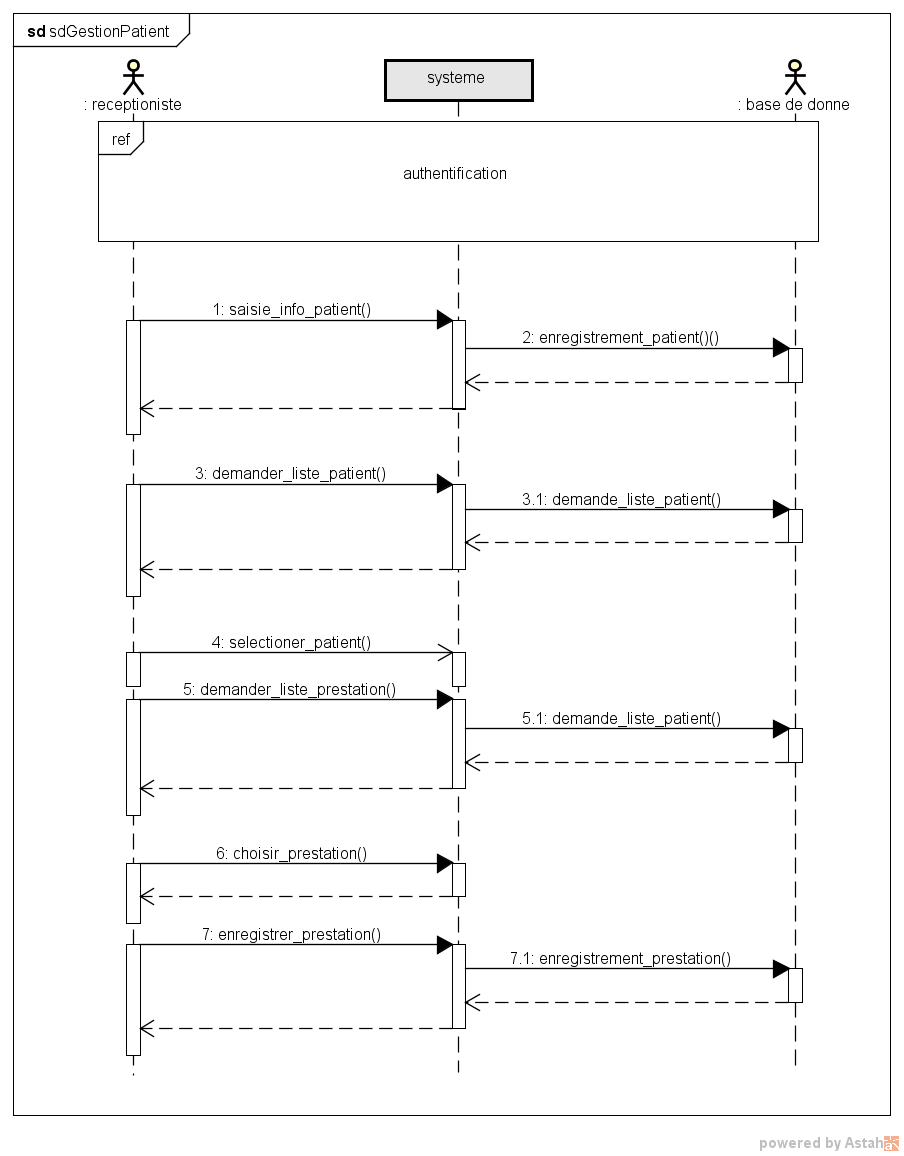
\includegraphics[scale=0.5]{Chapitre2/images/auth}
	  \caption{Diagramme de  séquence authentification}
	  	  \end{figure}
	  \newpage
	  
	  \subsection{Diagramme de séquence gestion patient}
	  \begin{figure}[h]
	  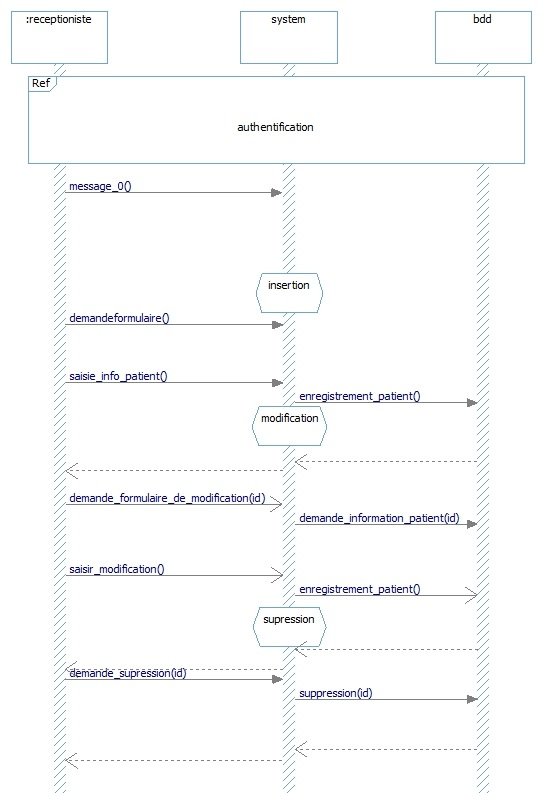
\includegraphics[scale=0.6]{Chapitre2/images/sd_gererpatient}
\caption{Diagramme de  séquence gestion patient}
	  \end{figure}
	  
	  \newpage
	  
	  \subsection{Diagramme de séquence gestion facturation}
	   \begin{figure}[h]
	  	  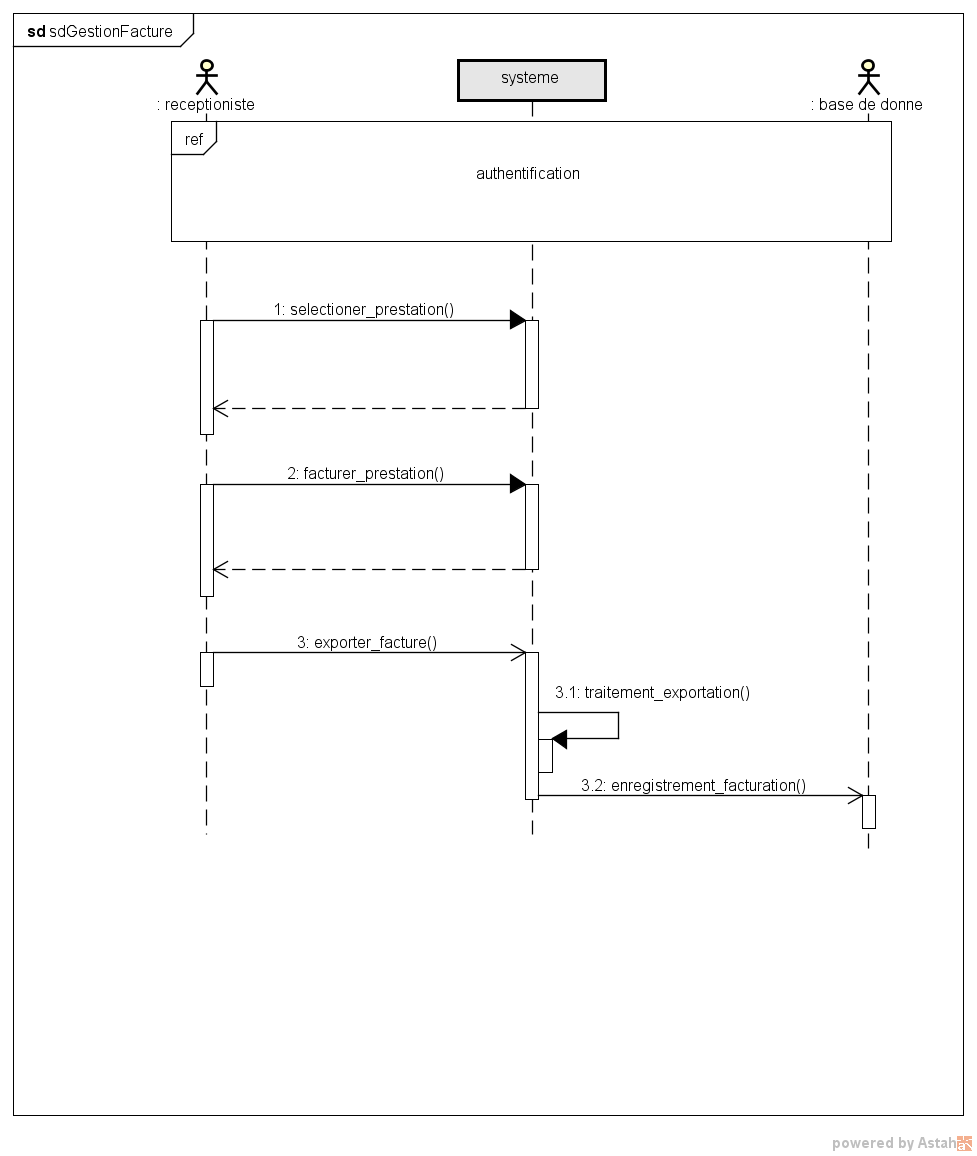
\includegraphics[scale=0.6]{Chapitre2/images/sd_gererfacture}
	  \caption{Diagramme de  séquence gestion facturation}
	  	  \end{figure}
	  
	  
	 
	
	  	  
	  \section{Diagramme de classe de l'application}
	  
	  \begin{figure}[h]
	  	  	  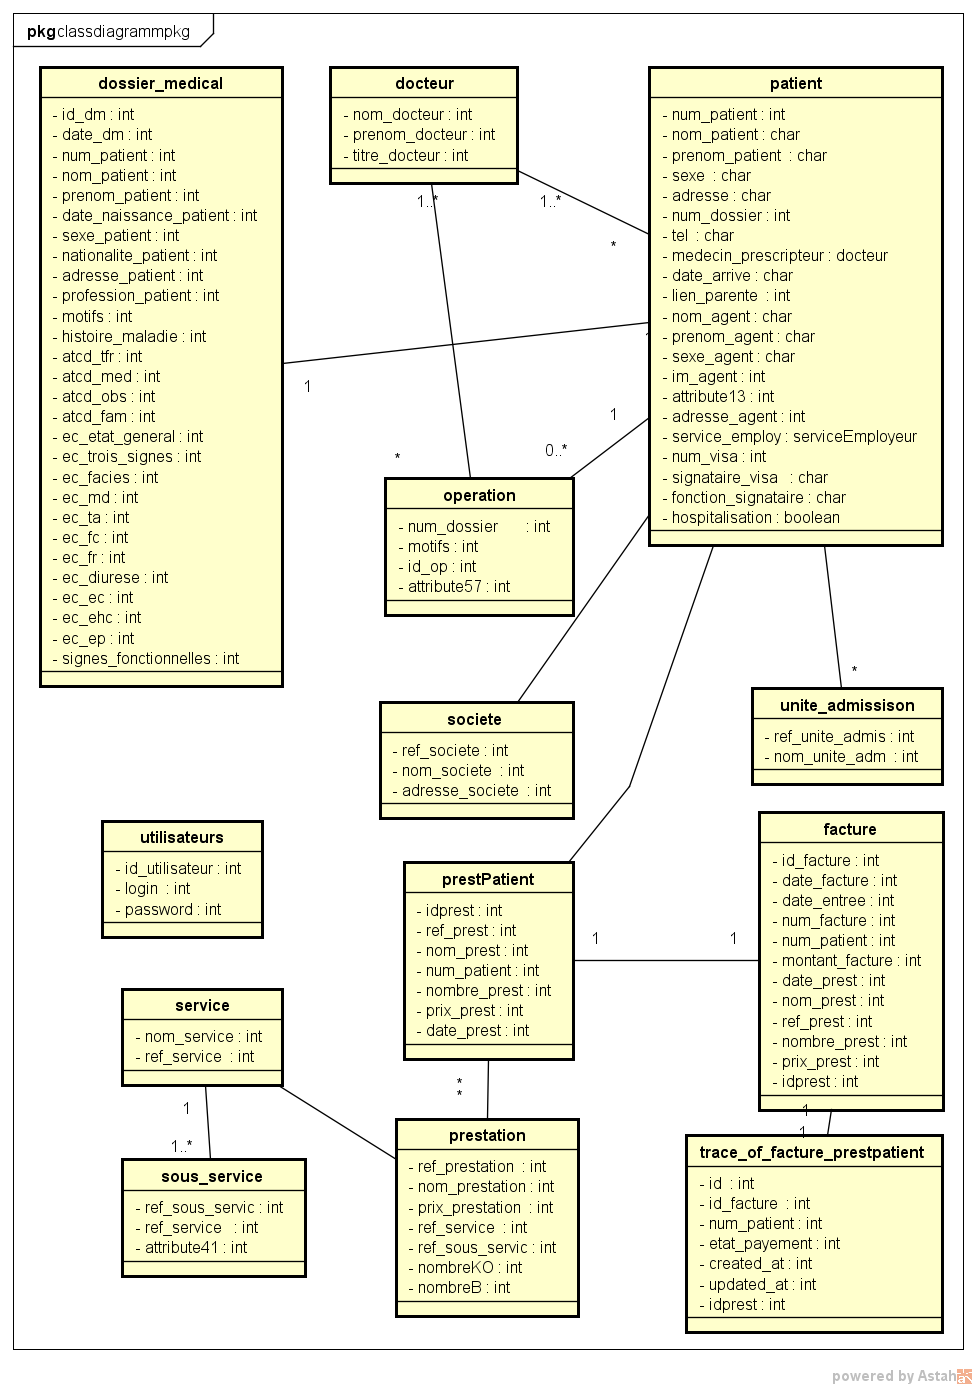
\includegraphics[scale=0.65]{Chapitre2/images/ClassDiagram0}
	  	  	  
	  	  	   
	  	  \caption{Diagramme de classe de l'application}
	  	  	  \end{figure}
	  
	  
	  
	  
	 
	  
	  
	  
	  